\chapter{Background \& Related Work}\label{ch:background}

\section{General Challenges of Computer Vision}

\subsection{The Semantic Gap}

One of the core insights of computer vision in general and content based image
retrieval in specific probably is that human perception is inseparably linked
to interpretation by the brain. As a human individual there is no way to
directly access visual information without them having been filtered and
weighted by one's personal experiences and cultural context. Therefore, when
people talk about visual similarity of images, it usually includes a large
degree of semantic similarity unconciously added to the perception. The
difference between that mode of perception and the current algorithmic ways to
analyse visual data has been eloquently coined \emph{the semantic gap} by
\autocite{smeulders_content-based_2000}:

\begin{quote}
The semantic gap is the lack of coincidence between the information that one
can extract from the visual data and the interpretation that the same data have
for a user in a given situation.
\end{quote}

Having had that realisation can guide the decision of a researcher or designer
of such systems.

\subsection{The Sensory Gap}

In addition to the semantic ambiguity described above, another major obstacle
of computer vision impacts a CBIR system: \emph{the sensory gap}. This term has
also been coined by \autocite{smeulders_content-based_2000}, where it's defined
as follows:

\begin{quote}
The sensory gap is the gap between the object in the world and the information
in a (computational) description derived from a recording of that scene.
\end{quote}

That terse definition includes a multitude of conditions, that can affect an
image, which a CBIR system operates on:

\begin{description}
    \item[Illumination] The brightness or direction of the illumination can
        hide or accent edges and texture properties in the scene. Similarly,
        the color of the illumination influences the recorded color information
        in the image.
    \item[Resolution] The imaging resolution sets a lower limit on the size of
        features that can be correctly recognised by any algorithm. As in all
        signal processing applications, aliasing of high frequency components
        of the image can introduce further ambiguities.
        \autocite{shannon_communication_1998}
    \item[Occlusion] Depending on the viewpoint of the recording and the
        composition of the scene, distinguishing parts of depicted objects may
        be occluded by other objects or objects may be only partially inside
        the recorded image.
    \item[Perspective] An object's proportions can be distorted by the imaging
        perspective.
\end{description}

An ideal CBIR system would use feature extraction and comparison methods that
can account and correct for such conditions.

\section{Anatomy of a CBIR System}

The inner workings of most CBIR systems can best be examined by looking at the
processing pipeline each query has to go through. The coarse sequence of
computational steps is almost the same in all such systems (Figure
\ref{fig:cbir_coarse_structure}):

\begin{enumerate}
    \item Acquire the image.
    \item Extract the signature using a feature extraction algorithm.
    \item Compare the signature to a database containing the signatures of the
        images to search within.
    \item Rank the images by similarity using the comparison results.
\end{enumerate}

\begin{figure}[h]
    \centering
    \subfloat[Local features]{%
        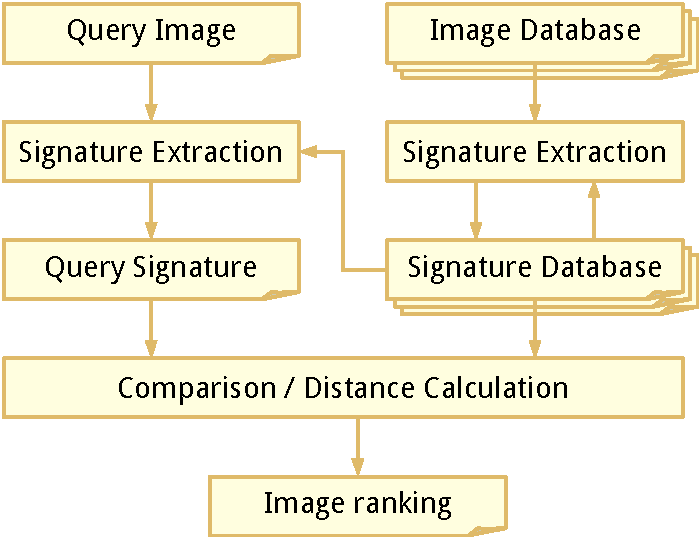
\includegraphics[width=0.45\textwidth]{cbir_anatomy_query_local_cropped}%
        \label{fig:cbir_coarse_structure_local}%
    }
    \quad
    \subfloat[Global features]{%
        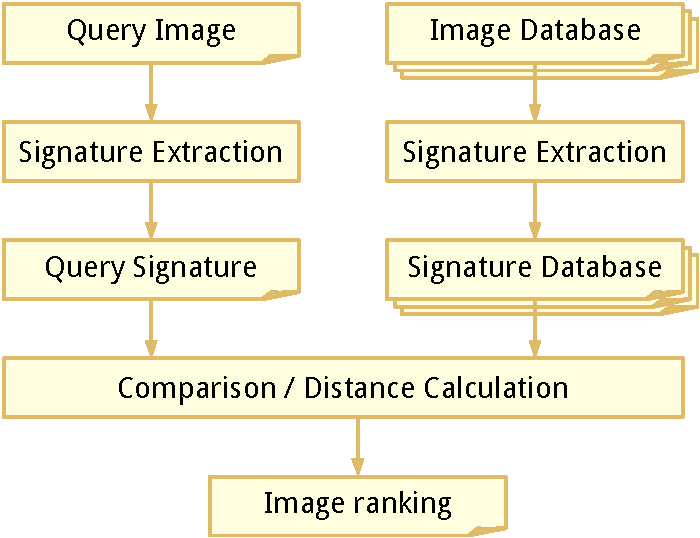
\includegraphics[width=0.45\textwidth]{cbir_anatomy_query_cropped}%
        \label{fig:cbir_coarse_structure_global}%
    }
    \caption{Coarse structure of a CBIR system}
    \label{fig:cbir_coarse_structure}
\end{figure}

\subsection{Image Aquisition}

TBD

\subsection{Signature Extraction}

TBD

\begin{figure}[h]
    \centering
        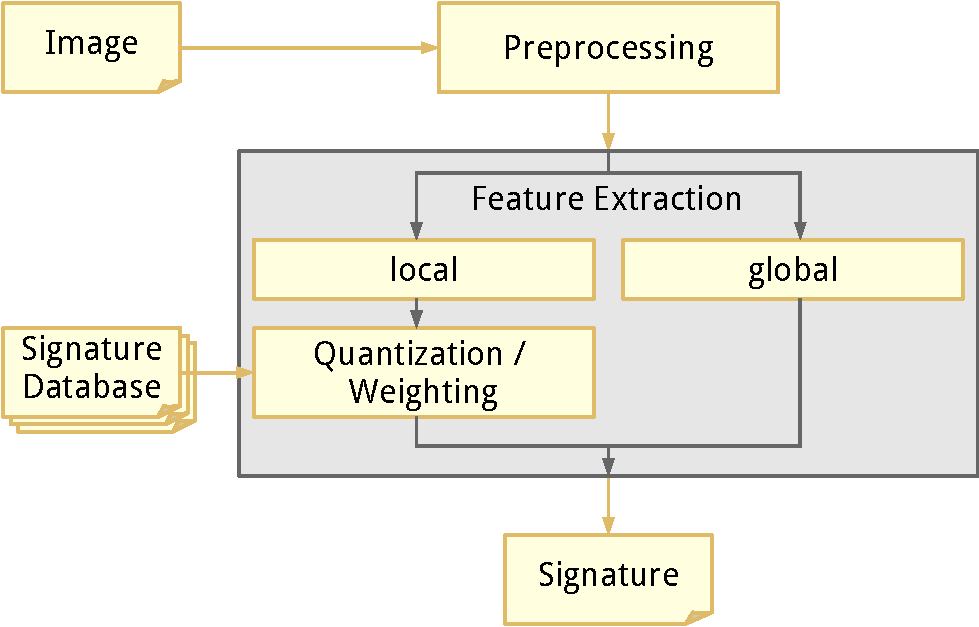
\includegraphics[width=0.8\textwidth]{cbir_anatomy_signature_extraction_cropped}
    \caption{Signature extraction in CBIR systems}
    \label{fig:cbir_signature_extraction}
\end{figure}

\subsection{Comparison and Ranking}

TBD

\section{Image Transformations for Feature Extraction}

Discuss FFT, Gabor Filters, HOG, SIFT/GIST

\subsection{The Continuous Curvelet Transform}

The formulation of the continuous curvlet transform (CCT) by Candes and Donoho
in \autocite{candes_curvelets:_2000} was based on Candes' previous definition and
expansion of the ridgelet transform \autocite{candes_ridgelets:_1998}. In that
publication they looked at the state of research into efficient representations
of edge discontinuities. They based their research on two realisations:
\begin{enumerate}
    \item A nonadaptive approach of signal approximation can compete with many
        of the adaptive schemes prevalent in previous research. At the same
        time the non-adaptivity comes with a greatly reduced computational
        overhead and reduced requirements for a priori knowledge. Obtaining
        that knowledge in the presence of blurred or noisy data can sometimes
        be unfeasable.
    \item Wavelet transforms can represent point singularities in a signal of
        up to two dimensions in a near-ideal manner, but fail to perform
        equally well on edges: Given a two-dimensional object in signal $f$, that
        is smooth except for discontinuities along a curve, a wavelet
        approximation $\tilde{f}^W_m$ from the $m$ largest coefficients
        exhibits an error of
        \begin{equation*}
            \| f - \tilde{f}^W_m \|^2 \propto m^{-1} \text{, for } m \rightarrow \infty
        \end{equation*}
        since up to $O(2^j)$ localized wavelets are needed to represent the
        signal along the edge. That falls short of what an approximation
        $\tilde{f}^T_m$ using a series of $m$ adapted triangles could achieve:
        \begin{equation*}
            \| f - \tilde{f}^T_m \|^2 \propto m^{-2} \text{, for } m \rightarrow \infty
        \end{equation*}
\end{enumerate}
They showed that a similarly precise approximation can be achieved by combining
Candes' ridgelet analysis \autocite{candes_ridgelets:_1998} with smart
windowing functions and bandpass filters. The steps of the transformation were
as follows:
\begin{enumerate}
    \item Decomposition of the signal into subbands of scale-dependent size
    \item Partitioning of each subband into squares
    \item Normalisation of each square to unit scale
    \item Analysis of each square in an orthonormal ridgelet system
\end{enumerate}

The result was a formulation of a decomposition that matched the parabolic
scaling law $width = length^2$ often observed in curves.

The above formulation became known as the curvelet 99 transform when Candes and
Donoho revised it soon after in \autocite{candes_new_2004}. The new version is
not dependent on ridgelets and aims to remove some shortcomings of the curvelet
99 transform, namely a simpler mathematical analysis, fewer parameters and
improved efficiency regarding digital implementations, which will be described
later.

The curvelet transform in $\mathbb{R}^2$ works by localising the curvelet
waveforms in the time domain. The "mother" curvelet waveform $\varphi_j(x)$ is
defined using two frequency domain windows $W(r)$, the "radial window", and
$V(t)$, the "angular window". A combined frequency window $U_j$ can then be
defined as
\begin{equation*}
    U_j(r, \theta) = 2^\frac{-3j}{4} W(2^{-j}r) V(\frac{2^{\lfloor\frac{j}{2}\rfloor}\theta}{2 \pi}).
\end{equation*}
If we then define $\varphi_j$ as being the inverse Fourier transform of
$\hat{\varphi}_j = U_j$, all curvelets of a scale $2^{-j}$ can be derived by
rotating $\varphi_j$ by ... and translating $\varphi_j$ by ....

%OLD STUFF BELOW

%Most approaches can be characterized by looking at three stages in their processing pipeline:

%\begin{description}
    %\item[Input format] The structure of the input data determines the amount of information available to the subsequent processing steps. Possible preprocessing steps include color space conversion, scaling and edge extraction.
    %\item[Extracted features] Many algorithms produce a large number of coefficients that can be reduced to a set of feature coefficients using by techniques such as vector quantization or principal component analysis (PCA).
    %\item[Distance metric] In order to rank the images according to similarity a metric is used to calculate the distance in feature space between two sets of feature coefficients. The selection of a metric is often closely coupled with the feature extraction algorithm.
%\end{description}

%\subsection{input format}
%Complete vs incomplete sketches, intra-/cross-domain

%\subsection{features}

%\begin{itemize}
    %\item bag of features from k-means clustered visual words [video google]
    %\item histogram of oriented gradients [chalechale + refs]
%\end{itemize}

%\subsection{metric}

%\begin{itemize}
    %\item after ranking using euclidean distance, rank by spatial similarity [video google]
    %\item Earth Mover's distance? [rubnerljcv00]
%\end{itemize}
